\maketitle
\chapter{BufferLine}
\section{Buffer e Pipeline: L'architettura Sliding Window}

La trasformazione di un immagine in un contesto spaziale bidimensionale è il compito principale del modulo \texttt{buffer\_line}. Questo blocco è responsabile della creazione della "finestra scorrevole" (Sliding Window) $3 \times 3$ necessaria per l'operazione di convoluzione.

\subsection{Architettura del Dataflow}
Il modulo implementa una struttura a registri a scorrimento (Shift Registers) interconnessi con buffer di linea (FIFO). L'obiettivo è rendere disponibili contemporaneamente, in un singolo ciclo di clock, i 9 pixel adiacenti necessari al filtro:

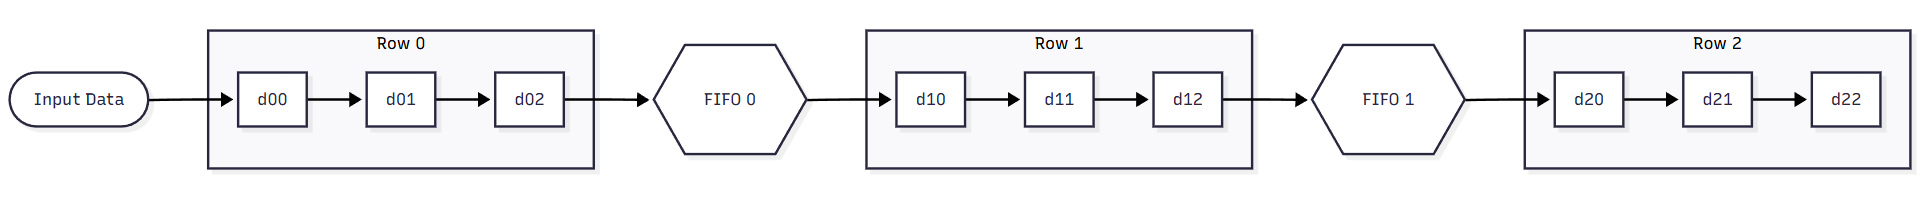
\includegraphics[width=\textwidth]{file_relazione/imgs/fifo.png}

\[
\text{Window} = \begin{bmatrix}
	d_{00} & d_{01} & d_{02} \\
	d_{10} & d_{11} & d_{12} \\
	d_{20} & d_{21} & d_{22}
\end{bmatrix}
\]
I dati in ingresso dall'interfaccia AXI-Stream vengono inseriti nel registro $d_{00}$. Ad ogni colpo di clock, se l'abilitazione della pipeline è attiva, i dati scorrono verso destra. Al termine della prima riga della finestra ($d_{02}$), il dato entra in un \textit{Line Buffer} che lo ritarda di un numero di cicli pari alla larghezza rimanente dell'immagine, per poi riapparire all'inizio della seconda riga ($d_{10}$).

Questa architettura garantisce che, una volta riempita la pipeline (latenza iniziale), i registri contengano sempre pixel spazialmente adiacenti, nonostante arrivino temporalmente sequenziali.

\subsection{Implementazione degli Shift Register Arrays}
Le FIFO necessarie per memorizzare le righe dell'immagine sono realizzate utilizzando array parametrici di vettori logici. La dimensione di questi buffer è critica e dipende dalla larghezza dell'immagine ($N_{col}$) e dalla dimensione del kernel ($K_{dim} = 3$).

La profondità del buffer è calcolata come:
\[
\text{Buffer Depth} = N_{col} - K_{dim} 
\]
Nel codice VHDL (Listing \ref{lst:linebuffer}), viene definito un tipo array per istanziare i due buffer di linea necessari per una finestra $3 \times 3$.

\begin{lstlisting}[language=VHDL, caption={Definizione e processo di shift dei Line Buffer}, label={lst:linebuffer}]
	-- Definizione dei tipi per il buffer
	-- Esempio: Image Width (32) - Window Size (3) = 29 elementi di buffer
	-- La dimensione e' parametrica basata su ncol
	type reg_array is array (ncol-4 downto 0) of std_logic_vector(7 downto 0);
	signal buffer1, buffer2 : reg_array;
	
	-- Processo di scorrimento (Line Buffer 1)
	process(clk)
	begin
		if rising_edge(clk) then
			if pipeline_en = '1' then
				-- Ingresso dal registro finale della riga precedente (d02)
				buffer1(0) <= d02_s;
			-- Shift dell'intera riga nel buffer
			for j in 1 to ncol-4 loop
				buffer1(j) <= buffer1(j-1);
			end loop;
	
			-- L'uscita del buffer alimenta la riga successiva (d10)
			d10_s <= buffer1(ncol-4);
		end if;
	end if;
end process;
\end{lstlisting}

\subsection{Gestione del Flush e Padding}
Una criticità nei filtri digitali è la gestione dei bordi dell'immagine. Quando l'ultimo pixel valido entra nella pipeline, la finestra di elaborazione non ha ancora terminato il suo lavoro: l'ultimo pixel deve infatti scorrere fino a raggiungere la posizione centrale ($d_{11}$) affinché l'operazione di filtraggio sia completa per tutto il frame.

Per gestire questa fase, il sistema implementa una logica di \textit{Zero Padding} attivata dallo stato di \textbf{FLUSH} della FSM.

\subsubsection{Logica di Inserimento Zeri}
Quando il segnale \texttt{flush} è attivo, l'ingresso fisico della pipeline viene disaccoppiato dall'interfaccia AXI e forzato a zero. Questo permette di "spingere" i dati validi residui attraverso i registri e i buffer di linea senza introdurre nuovi valori che corromperebbero il calcolo.

\begin{lstlisting}[language=VHDL, caption={Multiplexer di ingresso per gestione Flush e Padding}, label={lst:flush_logic}]
	if rising_edge(clk) and pipeline_en = '1' then
	-- Se siamo in fase di FLUSH, carichiamo zeri (Padding)
	-- per svuotare la pipeline dai pixel validi residui
	if flush_state = '1' then
		d00_s <= (others => '0');
	else
		-- Durante il normale funzionamento, acquisiamo il dato AXI
		d00_s <= s_axis_tdata; 
	end if;
	
	-- Shift dei registri di finestra (Row 0)
	d01_s <= d00_s;
	d02_s <= d01_s;
	end if;
\end{lstlisting}

Questa tecnica assicura che l'immagine in uscita abbia esattamente le stesse dimensioni di quella in ingresso, risolvendo il problema della latenza intrinseca della pipeline.